% !TEX root = main.tex

\chapter{Introduction}
\label{ch:intro}
\noindent

% breif overview
WebAssembly (Wasm)~\cite{wasm} is a low-level bytecode language that is safe, fast,
portable, and compact.
It is widely used as a compilation target for web applications.
Beyond web development, Wasm's advantages are also deployed in areas such as
edge computing~\cite{wasm-edge}, IoT~\cite{wasm-iot}, and
blockchain~\cite{wasm-block}.
% risk of implementation divergence
There are numerous Wasm engines, with all major browsers implementing their own
multi-tiered versions~\cite{v8, spidermonkey, webkit}.
Additionally, specialized engines target specific domains, such as embedded
systems and edge computing.
However, ensuring portability across these diverse implementations introduces
the risk of divergence among them.


% rigorous standardization -> spec is rigorous: formal notation & prose notation
To address this challenge, Wasm has been rigorously standardized by the
W3C~\cite{wasm-w3c}.
The Wasm specification is particularly rigorous, describing its semantics in
two complementary forms: formal notation and prose notation.
\red{\cref{fig:testop} illustrates the specification document for $testop$
instruction, where the upper part contains the prose notation, and the lower
part contains the formal notation.}
The formal notation employs mathematical rules to succinctly define the
semantics, supporting proofs such as type soundness.
Conversely, the prose notation uses pseudocode-like algorithms to explain the
semantics through step-by-step instructions.
Since most Wasm users and engine developers are less familiar with mathematical
formalism, they primarily rely on the prose notation.

\begin{figure}[t]
    \centerline{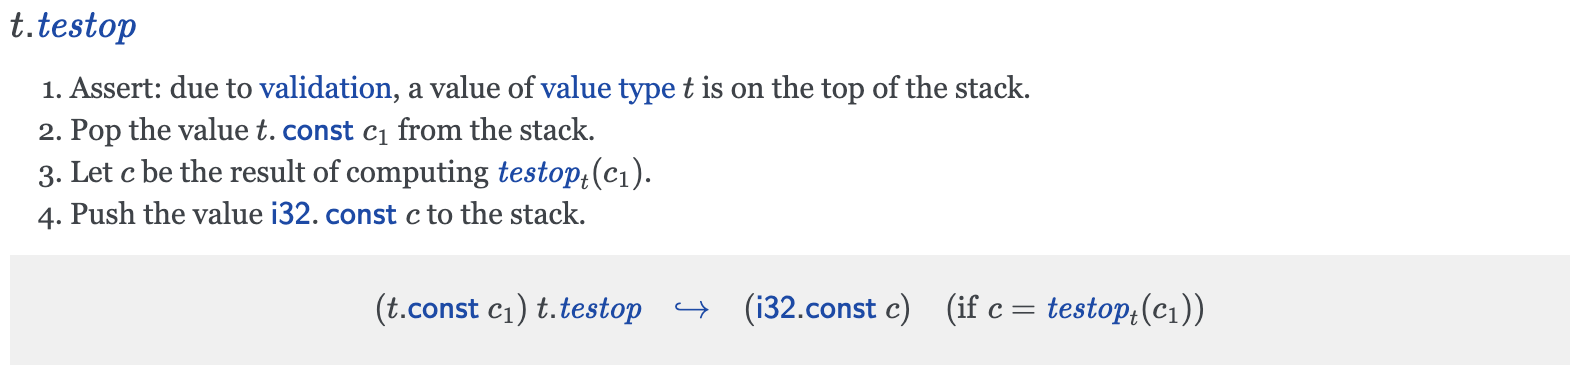
\includegraphics[width=15cm]{fig/testop}}
    \caption[Enter the caption title here]{\texttt{testop} instruction} \label{fig:testop}
    \centerline{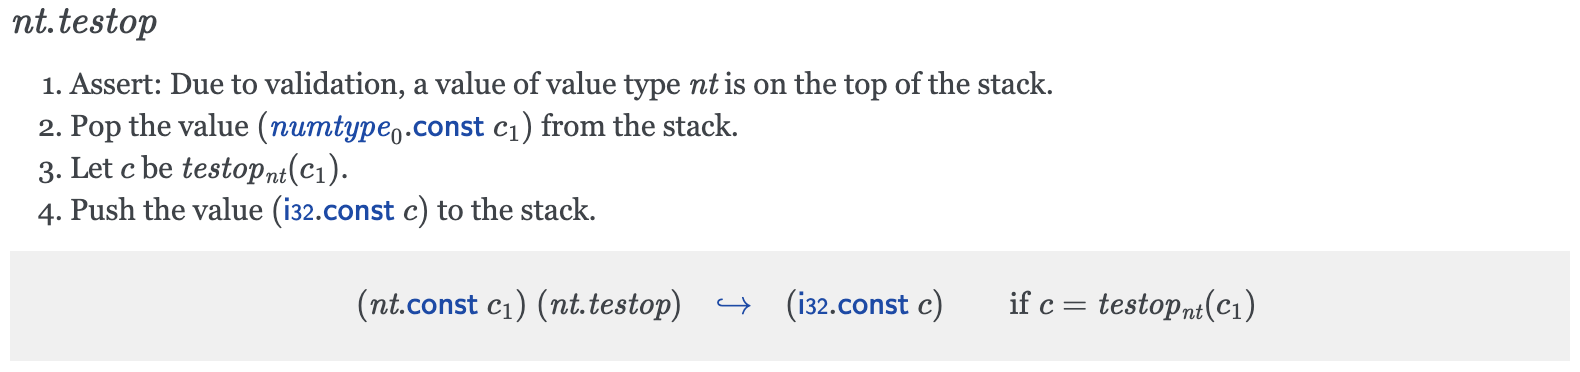
\includegraphics[width=15cm]{fig/spectec-testop}}
    \caption[Enter the caption title here]{SpecTec \texttt{testop} instruction} \label{fig:spectec-testop}
\end{figure}


% challenging specification process
The demanding standardization process places a significant burden on
specification authors.
Crafting this specification document is labor-intensive, and as Wasm evolves,
the manual effort required becomes increasingly challenging to scale.
Moreover, the dual requirement of maintaining both the formal notation and
prose notation exacerbates these difficulties.
The formal notation is written in LaTeX, and the prose notation is authored
in reStructuredText; neither of which is particularly user-friendly for
collaborative review.
This lack of accessibility in the specification's tooling increases the
likelihood of inconsistensies and errors, further complicating the
standardization effort.


% SpecTec
To mitigate this problem, we \red{propose} SpecTec, a framework for mechanizing
WebAssembly specification.
It provides domain specific language (DSL) that enables the declarative
definition of Wasm syntax and semantics, akin to the formal notation.
\red{
SpecTec performs type-checking on the DSL to prevent meta-level specification
errors and generates LaTeX for the formal notation.
Additionally, to capture the pseudocode-like structure of the prose notation,
SpecTec incorporates an imperative language, \textit{AL}, which stands for
Algorithmic Language.
SpecTec translates the DSL into AL and generate reStructuredText for the prose
notation.
\cref{fig:spectec-testop} is the specification document generated by the
SpecTec using the DSL and the AL.
The generated document closely resembles the official document except for some
minor notation changes and some missing hyperlinks.
One notable aspect of AL is that it is executable, meaning any specification
written in AL serves as a Wasm interpreter program.
By testing the Wasm interpreter program, we can check the correctness of the
specification.
This bridges the gap between formal specification and executable code.
Futhermore, SpecTec generates mechanized definitions for theorem provers.}


% challenge
\red{
One challenge of our approach is making AL executable.
Since the prose notation in the official specification is written in informal
pseudocode, the interpretation of the prose notation is not straightforward.
The naive implementation of AL interpreter produced incorrect results when
running Wasm official test suites, particularly those related to control flow.
}
Additionally, the absence of a formalized definition or formal semantics for AL
made it difficult to identify and address the fundamental issues in its design.
Since running tests is the primary method for assessing the correctness of the
specification, this limitation hindered the development of both the generated
interpreter and the specification itself.
This underscored the need for a more robust approach to formally define AL and
ensure its alignment with Wasm's complex semantics.


% solution
To address this, we present a formal model for how AL describes Wasm control flow.
Using this model, we identify the underlying issues and the necessary changes
to improve it.
Based on these insight, we formalize AL's syntax and semantics to accurately
capture Wasm control flow.
We then implement an AL interpreter according to this formalization and
evaluate its correctness.
The interpreter successfully passes all tests in the Wasm official test suite,
as well as tests from proposals.


% contribution
The contributions of this paper are as follows:
\begin{itemize}
  \item We propose a formal model for Wasm control flow in AL (\cref{ch:motivation})
  \item We formalize syntax and semantics of AL (\cref{ch:formal})
  \item We implement an AL interpreter based on the formalization (\cref{ch:eval})
\end{itemize}
